\documentclass{article}
\usepackage[utf8]{inputenc}
\usepackage{adjustbox}
\usepackage[utf8]{inputenc}
\usepackage[margin=1in]{geometry}
\usepackage{graphicx}



\title{TP3: Python Scrapping}
\author{Freile Mateo;Pedregal Juan Pablo }
\date{11/07/2021}

\begin{document}

\maketitle

\section{Ejercico 1}

El estudio de las fluctuaciones estacionales en los patrones delictivos se remonta a mediados del siglo XIX y sigue siendo un tema destacado en la literatura criminológica (Baron & Bell, (1976);Linning, S. J. (2015)). Un mejor entendimiento del cambio de la frecuencia de la tasa de crímenes en las diferentes etapas de un año, ayuda a implementar políticas públicas mas eficientes.\\

Existe una vasta cantidad de estudios que encuentran una relación positiva entre robos y temperaturas cálidas (Cohn, E., & Rotton, J. (2000);McDowall, D., Loftin, C., & Pate, M. (2012)).Estos patrones temporales a menudo se han atribuido al hecho de que las actividades de ocio de verano de las personas las alejan de sus hogares, eliminando así la tutela de su propiedad.De esta manera, se incrementan los incentivos y la utilidad esperada de cometer crimen.\\

Si bien no observamos una  tendencia decreciente en nuestro gráfico, tampoco se aprecia una fuerte correlacion positiva entre precipitaciones y hurtos en los hogares cada 10000 habitantes. No obstante, existe una tenue  correlación positiva, pero esto puede deberse al hecho de que tenemos  el promedio mensual de precipitaciones diarias.Nuestra hipótesis es que si tuviéramos la cantidad de precipitaciones y cantidad de hurtos diarios, podríamos llegar a encontrar la relación negativa preexistente en la literatura.\\


%Primera Imagen:

\begin{figure}[htbp]
\centerline{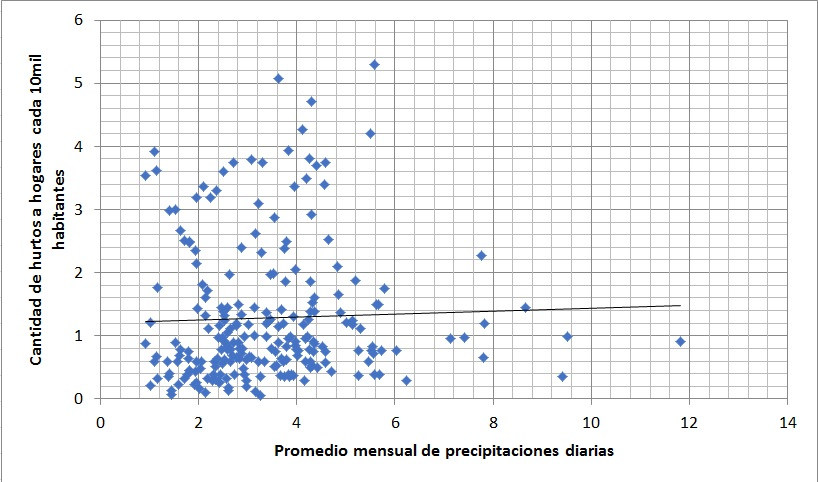
\includegraphics[scale=.8]{Precipitaciones_HurtosaHogares.jpg}}
\caption{Relación entre precipitaciones y hurtos a hogares}
\label{fig}
\end{figure}\\






\section{Ejercicio 2}
A continuación, queremos ver la correlación entre personas con tez negra y la cantidad de asaltos. Para ello, se  decidió graficar el porcentaje de personas con dichas  características sobre la población total y la cantidad de asaltos cada 10000 habitantes.\\

Como se puede observar en el gráfico, pareciera existir una tendencia positiva, indicando que a mayor porcentaje de personas de tez negra, mayor es la cantidad de asaltos en promedio para los 23 condados de Maryland con datos mensuales de 2015.\\

%Segunda Imagen:

\begin{figure}[htbp]
\centerline{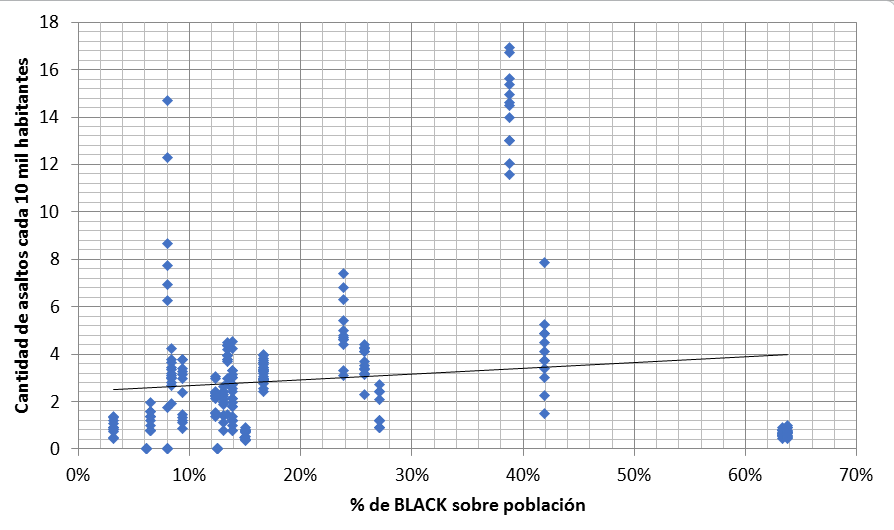
\includegraphics[scale=.8]{black_asaltos.png}}
\caption{Relación entre personas de tez negra y cantidad de asaltos}
\label{fig}
\end{figure}\\



\section{Bibliografía}
-Baron, R. A., & Bell, P. A. (1976). Aggression and heat: The mediating role of negative affect. Journal of Applied Social Psychology, 6, 18-30.\\
-Cohn, E., & Rotton, J. (2000). Weather, seasonal trends and property crimes in Minneapolis, 1987-1988. A moderator-variable time-series analysis of routine activities. Journal of
Environmental Psychology, 20, 257-272.\\
-Linning, S. J. (2015). Crime seasonality and the micro-spatial patterns of property crime in
Vancouver, BC and Ottawa, ON. Journal of Criminal Justice, 43, 544-555.\\
-McDowall, D., Loftin, C., & Pate, M. (2012). Seasonal cycles in crime, and their variability.
Journal of Quantitative Criminology, 28, 389-410.





\end{document}
